\section{Implementation}
I have successfully implemented software for transition from semantic representation to syntax as a proof of concept. I have chosen Church's algebra as algebraic structure the system. Basic operation of the algebra are: increment, assignment to zero, selection argument by specific index. Compositions are: application, primitive recursion, minimization.

On the input semantics solution is passed. The software parses semantic representation of solution into semantic tree according to rules choosen for semantics formalization. Leaves of the tree are input variables and constants and non-terminal vertices are compositions and metacompositions (compositions of compositions and operations).

It is selected JSON representation of the tree. Every vertex represented in fllowing form:\\
\texttt{
\{\\
\indent "name":character string,\\
\indent "id":numeric identifier,\\
\indent "static":[parameter list],\\
\indent "arguments":[{"no":1, "value":argument value},...]\\
\}\\
}

The \texttt{name} field is mnemonic designator of function, performed by specific vertex, \texttt{id} field is numeric vertex identifier for non-ambigous interpretation of vertices. \texttt{static} field is list of vertex parameters. They can be terms and/or values. Here term means semantic representation of other tree. Term may be an argument of compositions which are to manipulate them. The \texttt{arguments} field is a list of function(non-terminal vertex) arguments, in other words, list of vertices, which are connected to this one. Every element of list characterized by number \texttt{no} and value \texttt{value} which is vertex. A tree, which represents expression \texttt{add(IN0, mul(IN1, IN2))} looks like this:\\
\texttt{
\{\\
\indent "arguments": [\\
\indent \indent \{\\
\indent \indent \indent "value": "IN0",\\
\indent \indent \indent "no": 0\\
\indent \indent \},\\
\indent \indent \{\\
\indent \indent \indent "value": \{\\
\indent \indent \indent \indent "arguments": [\\
\indent \indent \indent \indent \indent \{\\
\indent \indent \indent \indent \indent \indent "value": "IN1",\\
\indent \indent \indent \indent \indent \indent "no": 0\\
\indent \indent \indent \indent \indent \},\\
\indent \indent \indent \indent \indent \{\\
\indent \indent \indent \indent \indent \indent "value": "IN2",\\
\indent \indent \indent \indent \indent \indent "no": 1\\
\indent \indent \indent \indent \indent \}\\
\indent \indent \indent \indent ],\\
\indent \indent \indent \indent "static": [],\\
\indent \indent \indent \indent "name": "mul",\\
\indent \indent \indent \indent "id": "384009"\\
\indent \indent \indent \},\\
\indent \indent \indent "no": 1\\
\indent \indent \}\\
\indent ],\\
\indent "static": [],\\
\indent "name": "add",\\
\indent "id": "415422"\\
\}
}

\begin{figure}
\centering
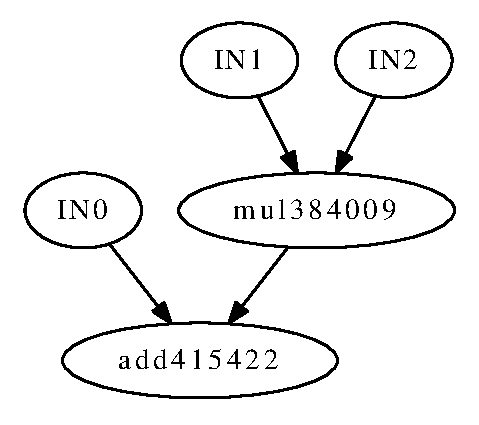
\includegraphics[width=2in]{source}
\caption{Graph representation of \texttt{add(IN0, mul(IN1,IN2))}}
\label{source_graph}
\end{figure}

\begin{figure*}
\centering
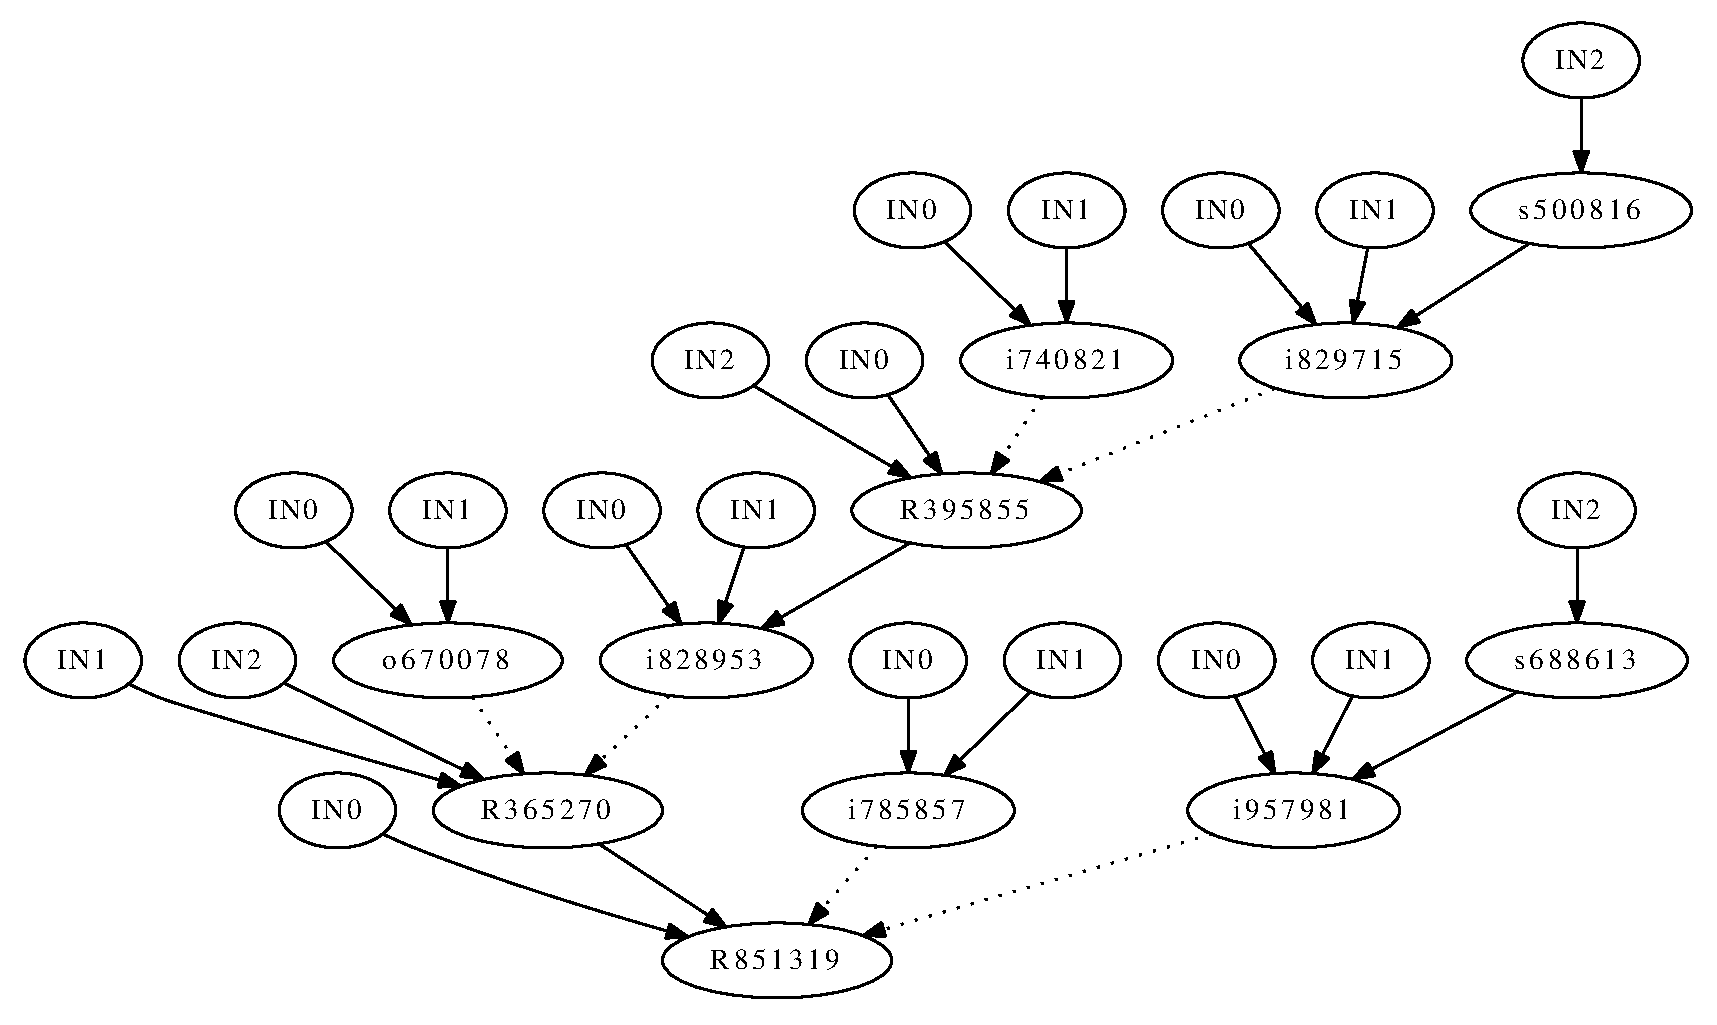
\includegraphics[width=5in]{primitive}
\caption{Graph representation of \texttt{add(IN0, mul(IN1,IN2))} after substitution.}
\label{primitive_graph}
\end{figure*}

For convenience the system produces tree representation of expression  (fig. ~\ref{source_graph}). It has some non-terminal vertices computer not familiar with, but algorithm of the system can replace them substituting instead non-familiar non-terminal vertices compositions of familiar ones(fig. ~\ref{primitive_graph}). Such compositions represented in JSON format too. For example operation of addition in terms of Church algebra:\\
\texttt{
\{\\
\indent name:R,\\
\indent id:\%ID1\%,\\
\indent static:[\\
\indent \{\\
\indent \indent name:i,\\
\indent \indent id:\%ID2\%,\\
\indent \indent static:[0],\\
\indent \indent arguments:[\\
\indent \indent \indent \{no:0, value:IN0\},\\
\indent \indent \indent \{no:1, value:IN1\}\\
\indent \indent ]\\
\indent \},\\
\indent \{\\
\indent \indent name:i,\\
\indent \indent id:\%ID3\%,\\
\indent \indent static:[2],\\
\indent \indent arguments:[\\
\indent \indent \indent \{no:0, value:IN0\},\\
\indent \indent \indent \{no:1, value:IN1\},\\
\indent \indent \indent \{no:2, value:\{\\
\indent \indent \indent \indent name:s,\\
\indent \indent \indent \indent id:\%ID4\%,\\
\indent \indent \indent \indent static:[],\\
\indent \indent \indent \indent arguments:[\\
\indent \indent \indent \indent \indent \{no:0, value:IN2\}\\
\indent \indent \indent \indent ]\\
\indent \indent \indent \indent \}\\
\indent \indent \indent \}\\
\indent \indent ]\\
\indent \}\\
\indent ],\\
\indent arguments:[\\
\indent \indent \{no:0, value:\%IN0\%\},\\
\indent \indent \{no:1, value:\%IN1\%\}\\
\indent ] \\
\}\\
}

Dotted lines on the figure~\ref{primitive_graph} denote that child vertex is a static parameter. Vertices with names starting with "o" are zero generators. Vertices with names starting with "s" perform operation of increment. Vrtices with name starting with "i" perform operation of selection one of arguments to send it to output, using static parameter, which denotes index of selected argument. Vertices with names starting with "R" represent primitive recursion composition. Terminal vertexes with names starting with "IN" represent arguments of the function in case when when a path from root to terminal vertex constists only of solid lines, in other case these are local inputs of compostion's static parameters.

The system produces HDL representation from such tree. To prove universality of the system, Moreover, generation of x86\_64 assembly was added as well. The system developed with Python programming language. It is agile enough to modify the system quickly.
